\chapter{Introduction}
\label{chapterlabel1}

\q{although the tracking of the B-field vector received over the S20 link is excellent, the quality and relevance of the resulting PAD can only be as good as the quality and relevance of the input data}\cite{owen2021}. 

- Chris Owen, 2021
\\

The Solar Orbiter Electron Analyser System instrument (EAS) is used to detect and characterise electrons in the solar wind. EAS can be commanded to follow various modes of operation depending on solar activity, spacecraft telemetry constraints, and other drivers. \q{Burst Mode} is a high-cadence operating mode that uses data from the Solar Orbiter Magnetometer instrument to make measurements at a timescale where electron plasma dynamics can be studied in particular detail. Unfortunately, the data transmitted from the magnetometer to EAS is of variable quality and relevance to the needs of EAS Burst Mode. The goal of the project described in this report is to investigate the quality and relevance of those transmitted magnetometer data, and the implications of their quality and relevance for EAS data products.
\\

The following sections provide a background to the project and a description of the project's goals in detail.
\newpage


\section{Solar Orbiter}
\begin{figure}[h!]
    \centering
    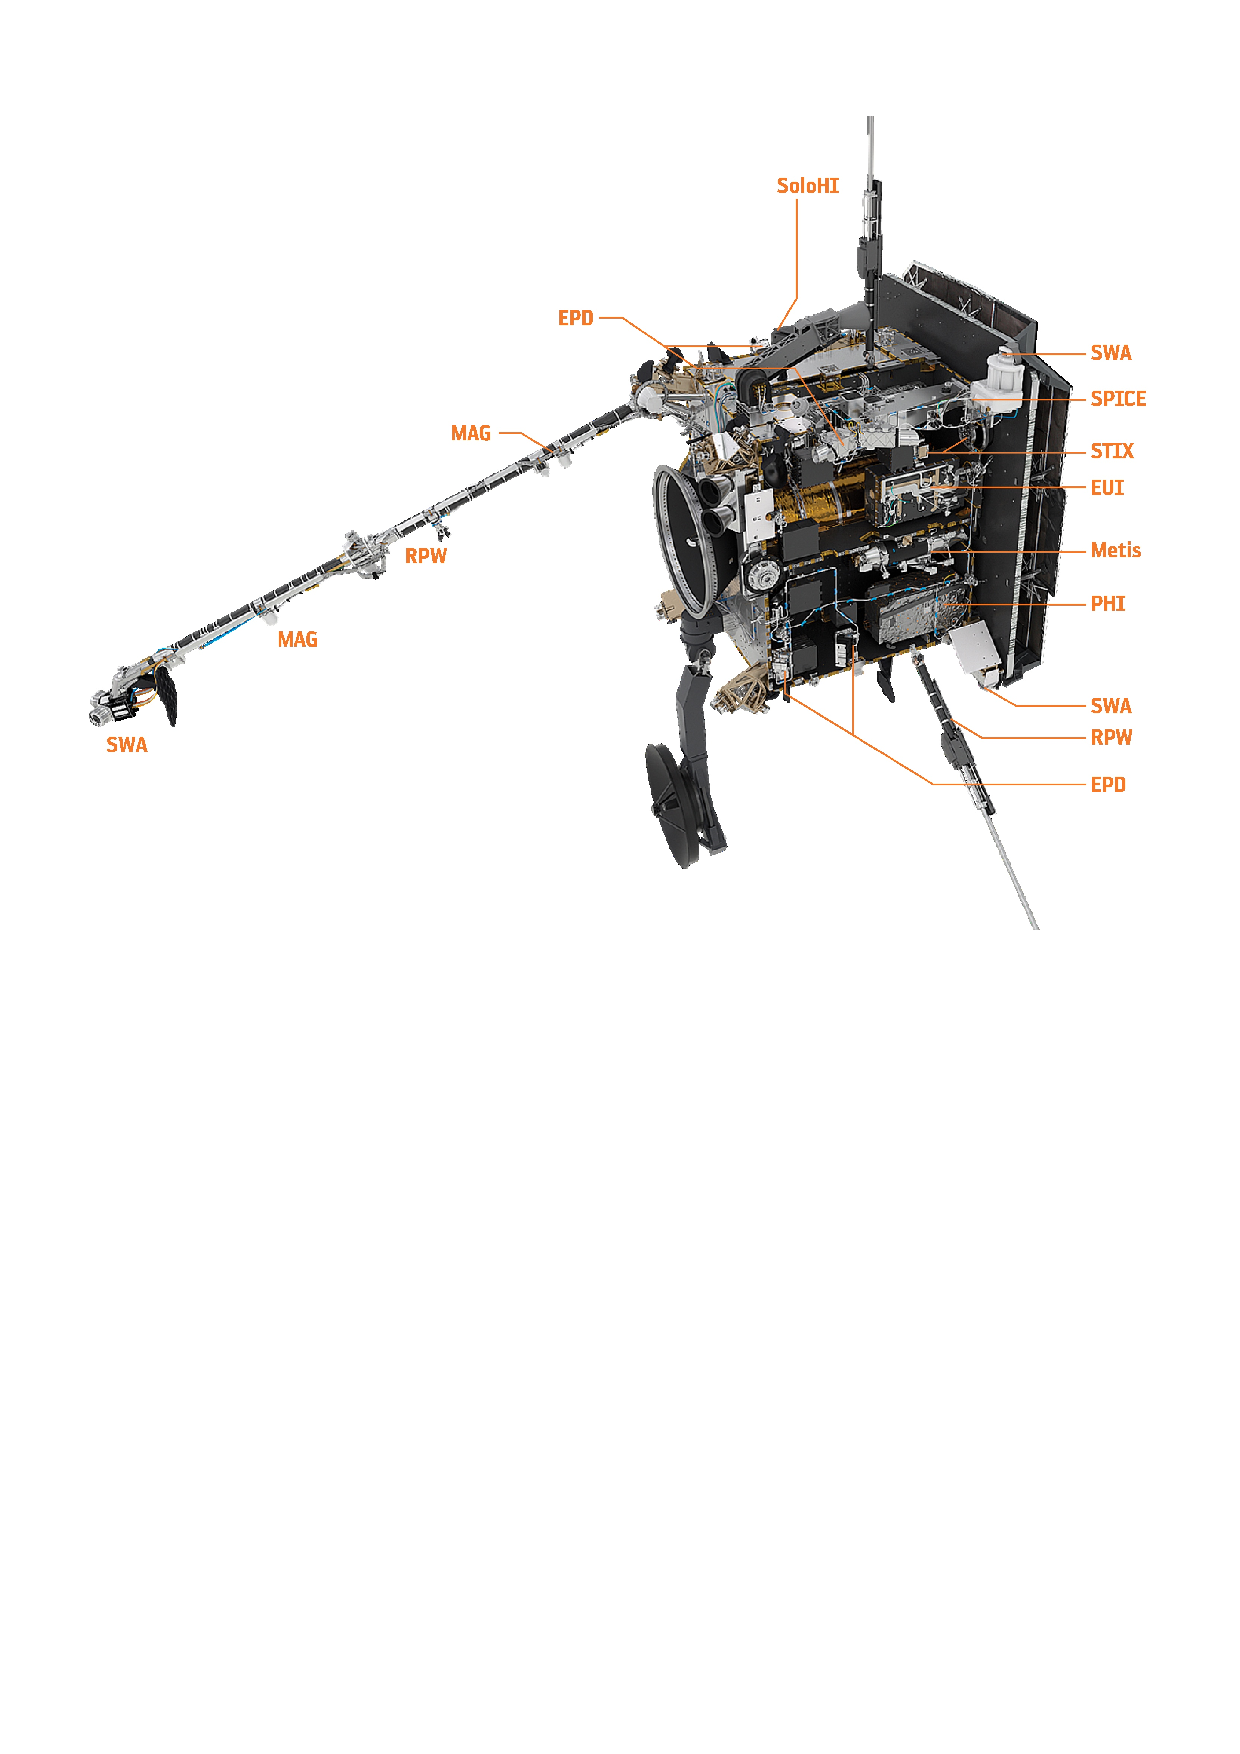
\includegraphics[width=1\linewidth]{figures/instruments.pdf}
    \caption{An image of Solar Orbiter with the -Y side panel removed to indicate the locations of onboard scientific instruments\cite{muller2020}. The boom is shown on the left-hand side of the image. Starting from the tip of the boom, in order of proximity to the spacecraft bus, the indicated instruments are SWA-EAS, MAG-OBS, RPW-SCM, and MAG-IBS\cite{horbury2020}\cite{maksimovic2020}. At the bottom right of the image is SWA-PAS, and at the top right is SWA-HIS\cite{owen2020}. }
    \caption*{Image Source: Müller et al\cite{muller2020}}
    \label{fig: instruments}
\end{figure}
\\

The overarching science objective of the Solar Orbiter mission is “How does the Sun create and control the Heliosphere – and why does solar activity change with time?”\cite{muller2020}. In service of this objective, the Solar Orbiter spacecraft carries a payload of scientific instrumentation along an inclined, eccentric solar orbit taking it to a perihelion of 0.28AU (\(\sim60\) solar radii), and up to 18\degree\ out of the ecliptic plane (extended mission phase may allow up to 30\degree). While the results from other heliophysics missions, including SOHO\cite{domingo1995}, HINODE\cite{kosugi2007}, STEREO\cite{kaiser2008}, and the Parker Solar Probe\cite{fox2016} have allowed the scientific community to make great strides towards answering similar questions to Solar Orbiter's overarching science objective, some gaps remain in our understanding of the inner heliosphere and the Sun's poles\cite{muller2020}. Solar Orbiter aims to fill those gaps.
\\

To that end, Solar Orbiter's instrumentation payload consists of a suite of remote sensing telescopes for purposes including solar wind and photospheric imaging and spectroscopy, as well as a suite of in-situ instrumentation for purposes including solar wind particle mass spectrometry and magnetic field sensing. These instruments are arranged around the spacecraft as illustrated in Figure \ref{fig: instruments}. Of particular interest to this project are the interactions between two of these in-situ instruments: The first is the Solar Wind Analyser Electron Analyser System (SWA-EAS or simply EAS); a sensor in the Solar Orbiter Solar Wind Analyser (SWA) suite of particle detectors. The second is the Solar Orbiter Magnetometer (MAG).

\section{SWA-EAS}

The Solar Wind Analyser suite comprises three in-situ particle sensors, each of which uses the well-established \q{top hat} electrostatic analyser design\cite{collinson2010}\cite{owen2020} to map incoming particles and their respective velocities/energies across each detector's field of view. The resulting maps allow the determination of the 3D \q{velocity distribution functions} (VDFs) for the particles within a given energy range over the measurement period. The three SWA sensors are: 

\begin{enumerate}
    \item The Heavy Ion Sensor (SWA-HIS or HIS), which produces VDFs for alpha particles and heavier ions in the solar wind to determine their relative charge states and abundances, not only at thermal energies, but also at \q{suprathermal} energies above the solar wind bulk speed\cite{mason2023}.
    \item The Proton-Alpha Sensor (SWA-PAS or PAS), which produces VDFs for solar wind protons and alpha particles, mainly at thermal energies.
    \item The Electron Analyser System, which produces VDFs for solar wind electrons at thermal and suprathermal energies.
\end{enumerate}

Working in concert, these sensors provide important data about local solar wind plasma to answer some of Solar Orbiter's more specific science questions, such as \q{What are the source regions of the solar wind and heliospheric magnetic field?}, \q{How do coronal mass ejections (CMEs) evolve through the corona and inner heliosphere?} and \q{How and where are energetic particles accelerated at the Sun?}\cite{owen2020}. Of the three SWA sensors, this project is most concerned with EAS. 
\\

\begin{figure}[h!]
    \centering
    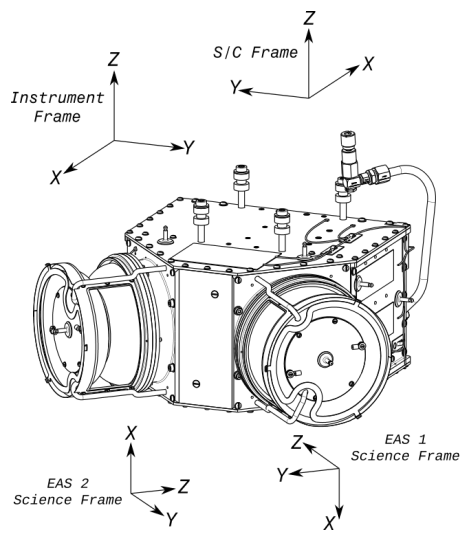
\includegraphics[width=0.75\linewidth]{figures/SWA-EA Sensor Heads.png}
    \caption{An annotated schematic depicting SWA-EAS as it appears on the end of the Solar Orbiter instrument boom (see Figure \ref{fig: instruments}), along with the axes of a few salient reference frames\cite{owen2021}. The spacecraft bus is towards the +X direction in the S/C (\q{spacecraft}) frame. The EAS1 sensor head (right) and the EAS2 sensor head (left) can be seen attached to a rectilinear electronics box.}
    \caption*{Image Source: Owen et al\cite{owen2021}}
    \label{fig: EAS schematic}
\end{figure}

EAS consists of two electrostatic analysers that inherit several aspects of their design from previous instruments such as the Cassini Plasma Spectrometer (CAPS) Electron Spectrometer (ELS)\cite{young2004}, the Mars Atmospheric and Volatile EvolutioN (MAVEN) Solar Wind Electron Analyser (SWEA)\cite{mitchell2016}, and the Cluster Plasma Electron And Current Experiment (PEACE)\cite{johnstone1997}. The two analysers, also called the \q{heads} of the instrument\cite{owen2021}, are orthogonal to each other as shown in Figure \ref{fig: EAS schematic}. Unlike HIS and PAS, which can afford relatively narrow, Sun-pointing fields of view (FOV) of 33° to +66° × ±20° and 24° to +42° × ±22.5° respectively, the EAS sensor heads each observe 360\degree\ of azimuth and ±45\degree\ of elevation in their respective reference frames (see \q{EAS 1/2 Science Frame} in Figure \ref{fig: EAS schematic}), theoretically covering more than the sky's full 4\(\pi\) steradians between them, where \(1.6\pi\) steradians are covered by the overlap between the two FOVs (see Figure \ref{fig: all bins})\cite{owen2020}. This FOV is required because, in comparison to protons and other ions, electron thermal velocities are expected to be much higher than the solar wind plasma bulk velocities. As a result, while protons and other ions are expected to enter their respective sensor primarily from the Sun-facing direction, electrons are expected to enter EAS more isotropically\cite{owen2020}. In reality, some of the EAS FOV is always obstructed by a set of support pillars and a shielding grid (to avoid spacecraft engine exhaust contamination) around each head, as well as the Solar Orbiter bus high-gain antenna and solar arrays\cite{owen2020}\cite{owen2021}\cite{dickson2024}. To minimise this obstruction, as well as to avoid electrostatic interference from the rest of the spacecraft,  EAS is positioned at the far end of the 4.4m Solar Orbiter instrument boom (see Figure \ref{fig: instruments})\cite{owen2020}\cite{olaskoaga2017}.
\\

\begin{figure}[h!]
    \centering
    \centerfloat
    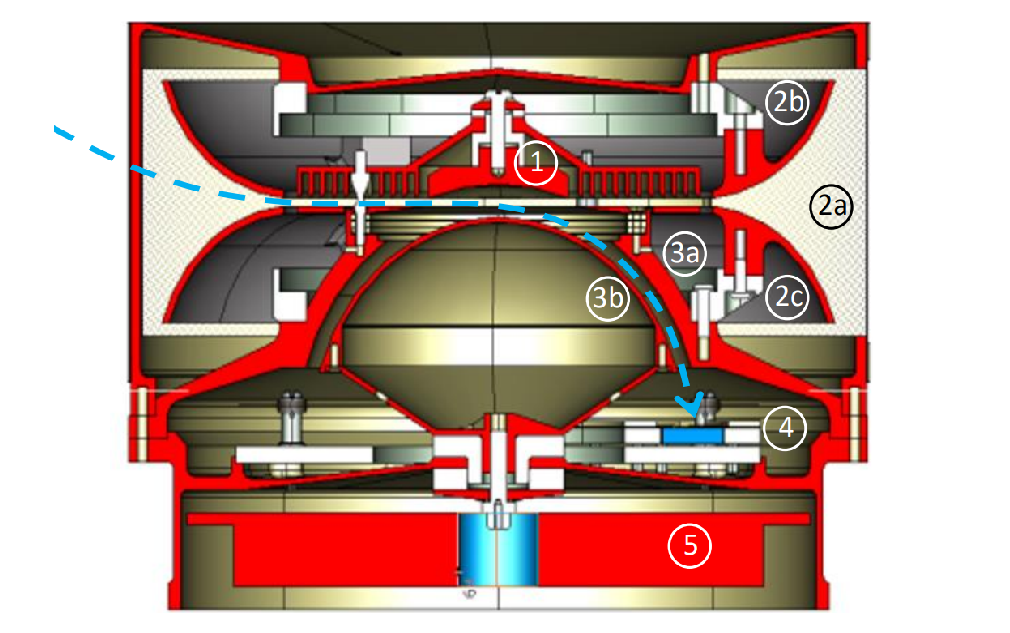
\includegraphics[width=0.85\linewidth]{figures/eas_cross-section.png}
    \caption{A diagram showing a cross-section of an EAS sensor head with an example electron trajectory illustrated in blue, and the following annotated subsystems\cite{owen2020}: (1) “top-cap” anode for controlling the geometric factor; (2) (a) sensor shielding grid; (2) (b,c) deflector electrodes for elevation selection; (3) (a,b) hemispherical electrodes for energy selection; (4) MCP subsystem; (5) charge amplifier integrated circuit.}
    \caption*{Image Source: Owen et al\cite{owen2020}}
    \label{fig: EAS cross-section}
\end{figure}

Ignoring obstructions, solar wind electrons can enter each sensor head from any elevation and azimuthal angle in its field of view. As they do so, the electrons fly through an electric field generated by a pair of deflector electrodes at the entrance of the head (subsystems 2b and 2c in Figure \ref{fig: EAS cross-section}). The electrodes are charged with positive voltages such that only incoming electrons from a narrow, selected range of elevation angles can continue through the sensor head. Electrons with elevations outside of this range will collide with the sensor walls and go undetected. This range corresponds to a single elevation angle bin. Electrons within the selected elevation range subsequently fly through a pair of hemispherical electrodes (subsystems 3a and 3b in Figure \ref{fig: EAS cross-section}). These electrodes create an electric field that only allows electrons within a narrow, selected range of velocities/energies to continue to the detector proper, filtering the electron population again. This range corresponds to a single energy bin. If an electron passes through these electron optics, then its trajectory ends when it impinges on a segment of an annular microchannel plate (MCP) corresponding to its azimuthal angle (subsystem 4 in Figure \ref{fig: EAS cross-section}). As a result, the incoming electron induces the emission of \(2\times10^{6}-5\times10^{6}\) secondary electrons which collect at the MCP anode, resulting in a characteristic voltage pulse that triggers a detection\cite{owen2020}.
\\

During EAS operation, the deflector electrodes sweep through up to 16 elevation bins, sequentially, in the range of ±45\degree. The elevation bins are unequally sized according to a\footnote{SWA-EAS has used different elevation bin tables at different times over the course of the Solar Orbiter mission. Due to an error in the EAS data acquisition pipeline discovered during this project, this table has occasionally been incorrect (see Section \ref{sim steering}).} table of voltages aboard Solar Orbiter, which is designed to account for increasing angular resolution at increasing deflection angles, with bin widths varying from \(\sim2\degree\) to \(\sim10\degree\). For each elevation bin, the hemispherical electrodes sweep through up to 64 logarithmically-spaced energy bins, sequentially, in the range \([\sim1\textrm{eV},\sim5\textrm{keV}]\). The full range of 0-360\degree\ of azimuth is split into 32 equally-spaced azimuthal bins, all of which are sampled simultaneously for each combination of elevation and energy. The result is a distribution of solar wind electron energies per solid angle; an electron VDF.
\\

\section{MAG}
The Solar Orbiter magnetometer consists of two three-axis fluxgate magnetometers located on the Solar Orbiter instrument boom. The inboard sensor (MAG-IBS) and outboard sensor (MAG-OBS) respectively (see Figure \ref{fig: instruments}).  The two sensors are at different positions along the boom to minimise the risk of magnetic contamination by the rest of Solar Orbiter both by distance attenuation and by subtracting the effect of Solar Orbiter through magnetic gradiometry. The design of MAG borrows heavily from that of previous magnetometers flown on the Cassini\cite{dougherty2004} and Double Star\cite{carr2005}, missions, and forms the basis for future magnetometers on missions including IMAP\cite{mccomas2018}\cite{dickson2024}. The author has previously described the operation of a fluxgate magnetometer as follows\cite{dickson2024}: 

Each magnetometer consists of two orthogonal fluxgate ring-cores (one of which is partially visible in Figure \ref{fig: magnetomato}). The fluxgate cores consist of three copper windings; One inner “drive” winding and two outer, orthogonal, “sense” windings. The inner “drive” winding is wound around a ring of magnetically-permeable material which it drives into successive states of oppositely-polarised magnetic saturation at the “drive frequency” through magnetic induction. In an environment with no external magnetic field, the magnetic field induced in one half of the ring is designed to perfectly counteract the antisymmetric field induced in the opposite half, resulting in zero magnetic field in the ring overall. However, if an external magnetic field is present and oriented along the plane of the ring, then the drive winding will drive the ring core into magnetic saturation more quickly in the direction parallel to the external magnetic field and more slowly in the direction antiparallel to the external magnetic field. The effect of such an external magnetic field is to temporarily break the symmetry of the induced magnetic field in the ring core, causing a pulse of magnetic flux density which repeats at twice the drive frequency. These pulses induce voltages in the outer sense windings from which a 2D external magnetic field vector can be recovered. With two orthogonal ring-cores, each fluxgate magnetometer can recover an external magnetic field vector in full 3D\cite{horbury2020}\cite{dickson2024}. 
\\

\begin{figure}[h!]
    \centering
    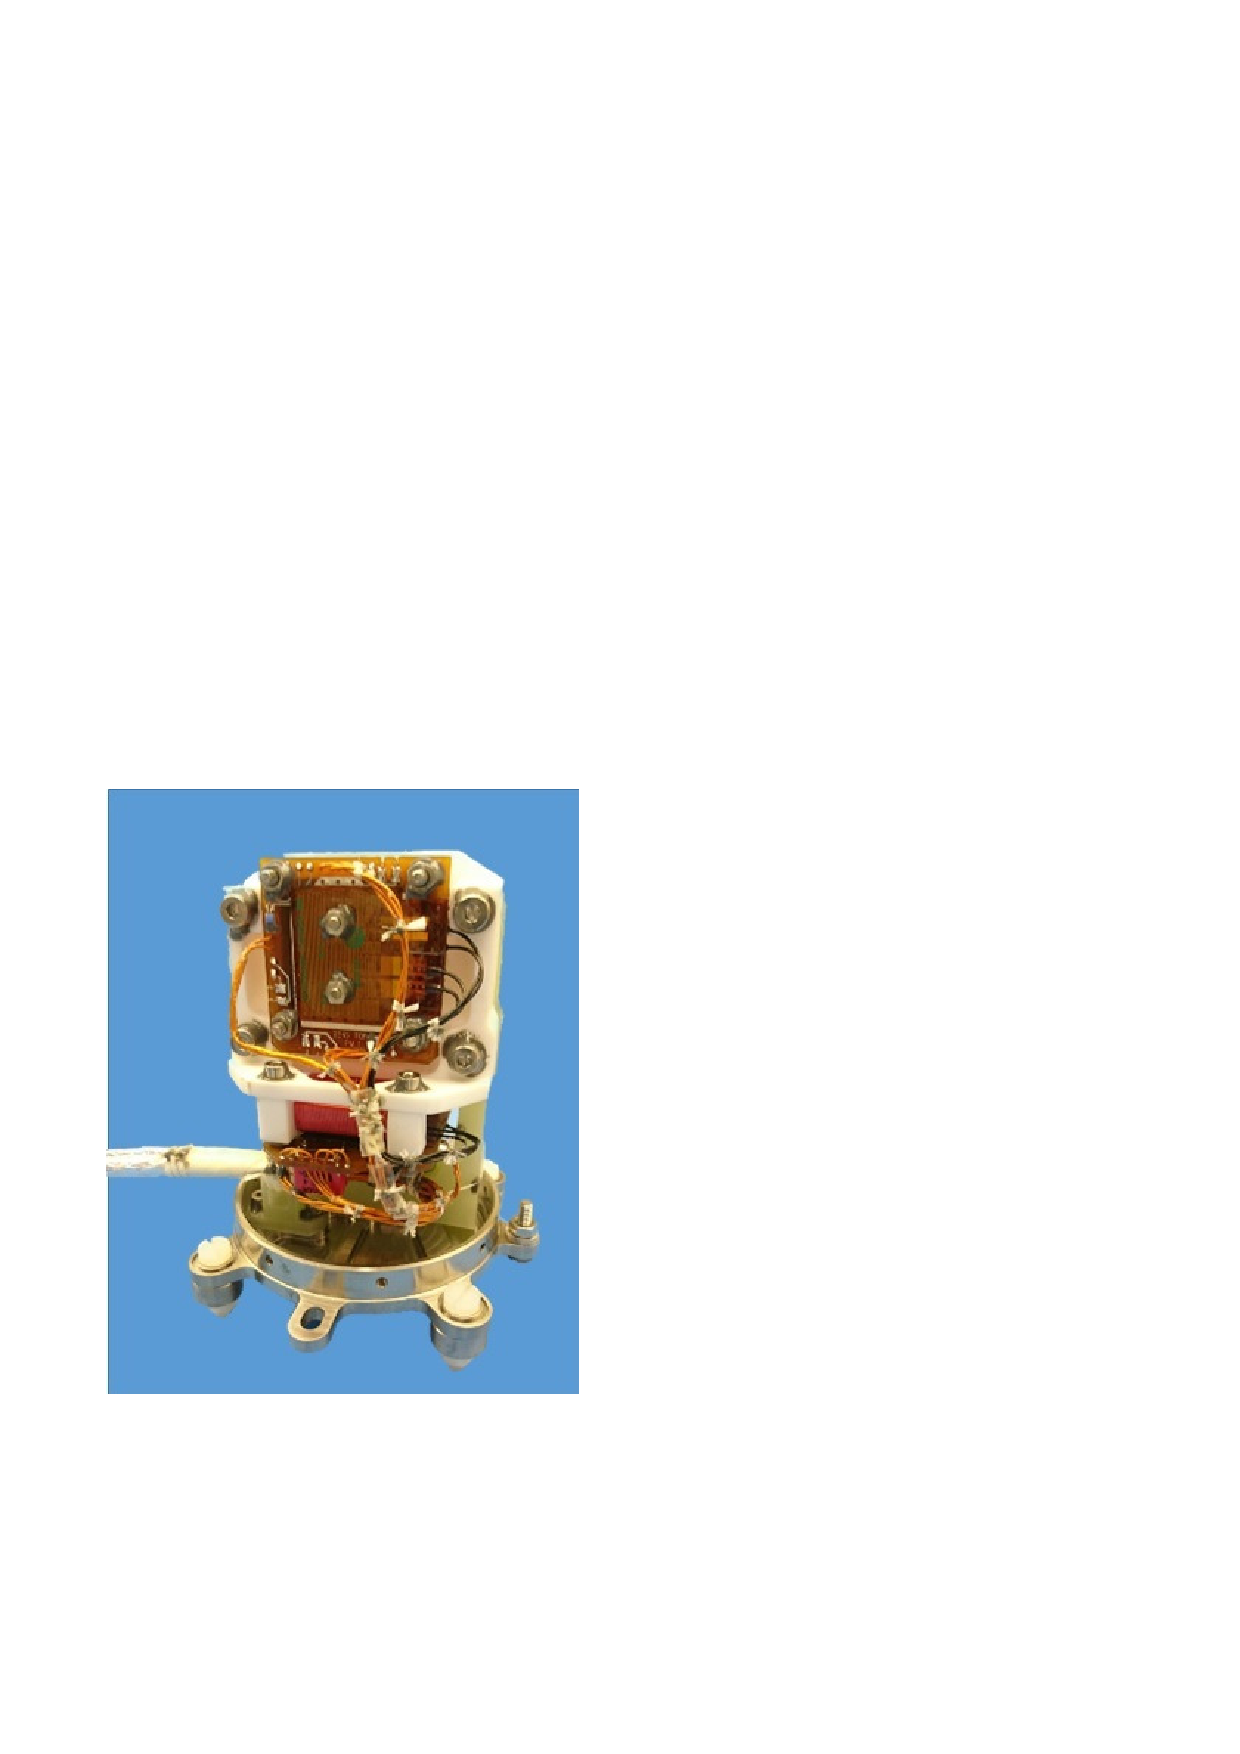
\includegraphics[width=0.5\linewidth]{figures/magnetomato.pdf}
    \caption{An image of one of the Solar Orbiter fluxgate magnetometer sensors as seen in the lab with its protective radiation shield removed\cite{horbury2020}. One ring core with its bright red outermost sense winding can be seen mounted on the underside of a white, ceramic bracket. The other core is unseen, mounted on the other side.}
    \caption*{Image Source: Horbury et al\cite{horbury2020}}
    \label{fig: magnetomato}
\end{figure}


The measured values of the axial components of the external magnetic field vector are known to occasionally “drift” due to imperfections in the magnetometer hardware, leading to offsets that affect magnetic field vector orientation. These offsets are corrected through data processing on the ground and through occasional updates to the software aboard Solar Orbiter\cite{horbury2020}. The central issue in this project is the effect of onboard MAG data inaccuracies, including offset, on EAS pitch angle data. 

\section{EAS Pitch Angle Distributions} \label{EAS PAD}
A particle's pitch angle, often denoted \(\alpha\), is the angle between the particle's velocity vector \(v\) and the local magnetic field vector \(B\). \(\alpha\) is given by:

\begin{equation} \label{eq: pitch angle}
    \alpha=\arctan{\frac{v_\perp}{v_\parallel}}
\end{equation}

where \(v_\parallel\) and \(v_\perp\) are the particle's velocity components parallel and perpendicular to \(B\) respectively\cite{pilipp1987}. Analysis of electron pitch angle distributions (PADs) has revealed distinct electron populations in the solar wind. Some populations have a tendency to collide amongst themselves, resulting in a \q{thermal} distribution with mainly isotropic pitch angles that  can be modeled, to within a close approximation, by a Maxwell-Boltzmann distribution. These represent the \q{bulk} of the electron plasma. Other populations are more anisotropic, forming narrow electron beams with pitch angles that may be field-aligned, making up the so-called  electron \q{strahl}. These anisotropic electrons tend to collide less frequently, so their trajectories are less uniformly distributed\cite{pilipp1987}\cite{marsch2006}.
\\

\begin{figure}[h!]
    \centering
    \centerfloat
    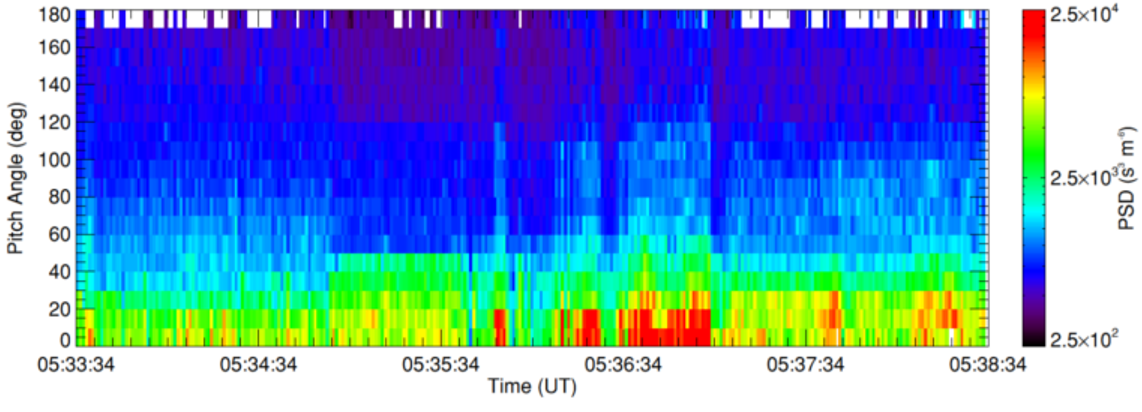
\includegraphics[width=1.1\linewidth]{figures/PADexample.png}
    \caption{Pitch angle data recorded by Solar Orbiter SWA-EAS in Burst Mode over 5 minutes on 26th June 2020\cite{owen2021}. Electron counts are plotted as a PSD. Time is plotted in Universal Time. Electron pitch angle is plotted in degrees.}
    \caption*{Image Source: Owen et al\cite{owen2021}}
    \label{fig: PAD example}
\end{figure}

An example PAD generated using Solar Orbiter SWA-EAS data is shown in Figure \ref{fig: PAD example} for a 5-minute period starting at 05:33:34 UT on 24th June 2020\cite{owen2021}. Shown here is the phase space density, or concentration, of strahl electrons with energies \(>70\)eV. The concentration is presented in terms of power spectral density (PSD) in colours from black (fewest electrons) to red (most electrons)\footnote{White pitch angle bins on this plot represent missing data, relating to each PAD's completeness score, which will be important in Section \ref{completeness}.}. A different PAD is plotted at every 1/8th-second time step (corresponding to EAS Burst Mode; see below). Notice that, for each time step, only pitch angles are shown from 0\degree\ to 180\degree\. It may seem that a full map of the sky would be required to fully capture electron concentrations at different phase angles about the local magnetic field at a given pitch angle, implying \textit{two} angles in spherical coordinates for every time step. However, near this time resolution, it is expected that any instantaneous in-homogeneities in electron concentration at different gyrophase angles about the local magnetic field will disappear too quickly to discern, such that the concentration at all phase angles for a given pitch angle can be assumed to be uniform; in a state of so-called \q{gyrotropy}\cite{owen2021}. This is expected to be a safe assumption at this timescale\cite{vocks2012}\cite{spinnangr2022}\cite{owen2021}. This can be understood because the expected electron gyroperiod in the solar wind at \(\sim\)1AU is much shorter than the 1/8th-second timescale. Assuming magnetic field strength \(B\approx1\textrm{nT}\), then the electron gyrofrequency \(\omega_{e}\) is given by:

\begin{equation} \label{eq: gyrofreq}
    \omega_{e}=\frac{eB}{m_{e}}=\frac{e\times10^{-9}}{m_{e}}\approx176\textrm{ rad/s}
\end{equation}

where \(m_{e}\) is the electron mass. The corresponding gyration frequency is therefore \(\omega/2\pi\approx28.0\textrm{/s}>>8\textrm{/s}\). Therefore, if this is a realistic estimate, then over a single 1/8th-second measurement, most electron agyrotropy is expected to be thoroughly averaged and rendered indiscernible. Lu et al 2020 has similarly supported the assumption of  gyrotropy when using 1/4th-second time steps in 2D particle-in-cell simulations of magnetic reconnection at Earth, on the basis that the local electron gyroradius should be comparable in size to the local plasma ion skin depth - should this be analogous to the EAS environment with the solar wind's plasma parameters to within an order of magnitude, then the assumption of gyrotropy for EAS is expected to be safe\cite{lu2020}\cite{lu2019}.
\\

The PAD in Figure \ref{fig: PAD example} was taken while EAS was operating in \q{Burst Mode}, which differs from the more typical \q{Normal Mode} in that it generates PADs \(\sim8\times\) faster. A description of Normal Mode and Burst Mode PAD determination follows.



\subsection{EAS Normal Mode} \label{EAS Normal Mode}

Most EAS data are collected in normal mode, where all 64 energy bins, 16 elevation bins, and 32 azimuth bins are sampled, yielding as close to a full-sky VDF as possible. The 32 azimuth bins are sampled simultaneously. Sampling a single energy bin for a single elevation bin takes \(\sim0.96\)ms\cite{owen2021}. Therefore, cycling through all energy and elevation bins in sequence takes \(64\times16\times0.96\textrm{ms}=0.983\textrm{s}\approx1\textrm{s}\), yielding Normal Mode data at a data rate of \(\sim1\)Hz\cite{owen2021}. The pipeline involved in acquiring a VDF and a subsequent PAD in Normal Mode can be summarised as follows\cite{owen2020}:

\begin{enumerate}
    \item Acquire a full-sky EAS VDF with 64 energy bins \(\times\) 16 elevation bin \(\times\) 32 azimuth bins at 1Hz,
    \item Acquire a MAG vector at 1Hz,
    \item Downlink EAS VDF and MAG vector to ground,
    \item Post-process MAG vector on ground, applying any necessary corrections,
    \item Combine EAS VDF and MAG vector to yield a PAD.
\end{enumerate}

For a more detailed description, consider Figure \ref{fig: all bins}. This figure shows the combined elevation and azimuth bin \q{pixels} available to each EAS sensor head (EAS1 in blue and EAS2 in red) projected on to a map of the full sky in spherical, spacecraft reference frame (SRF) coordinates where [0,0] points directly away from the Sun, and +90\degree\ elevation points out of the ecliptic plane. This amounts to a total of \(16\time32=512\) pixels per head. In normal mode, an EAS head first samples electrons from all of the pixels in its FOV. Meanwhile, MAG samples the local 3D magnetic field vector in its own Burst Mode (128Hz) or Normal Mode (8Hz)\cite{horbury2020}. Now, consider Figure \ref{fig: normal - full contours}, where a magnetic field vector from the same period as the 1s PAD is superimposed onto a projection of the EAS1 bins in SRF coordinates. Here, the green diamond represents the vector parallel to the magnetic field (i.e. the B-vector itself), and the green square represents the antiparallel vector. Surrounding the parallel vector are various contours of constant pitch angle at every 15\degree\ in the range \([0\degree,180\degree]\). To aid explanation, let the vectors in Figure \ref{fig: normal - full contours} represent the ground magnetic field post-processing\footnote{In reality, this vector was taken from data from the archive corresponding to the unprocessed magnetic field transmitted over the S20 data link in EAS Burst Mode (see Section \ref{EAS Burst Mode}). In this case, it is only treated as an analogy for the ground magnetic field.}. In this case, wherever an EAS pixel is crossed by a pitch angle contour, that pixel has sampled electrons with the contour's pitch angle. Calculating the pitch angle for every pixel in the 3D VDF allows a 2D PAD to be constructed for every azimuthal bin, each of which corresponds to a range of gyrophase angles. By combining samples from all the azimuthal bins in post-processing (this is harmless under gyrotropy), the gyrophase dimension is collapsed, yielding a single, 2D PAD for the 3D VDF.
\\

Even with compression, the volume of data implied by a full-sky, 3D VDF in Normal Mode has significant implications for the SWA telemetry budget, limiting full-cadence (1s/sample or 1Hz) data downlink to a 5-minute period per day. Instead, the SWA Data Processing Unit (SWA-DPU) typically downlinks moments of full VDFs at a cadence of 4s/sample, and full VDFs are limited to 10s/sample or 100s/sample cadences when downlinked. The limited telelmetry budget places even more constraints on what is already a relatively low cadence for measurements of solar wind electron dynamics (baseline of 1s/sample), motivating the design of a faster and less data-intensive method of operation; EAS Burst Mode.

\begin{figure}[h!]
    \centering
    \centerfloat
    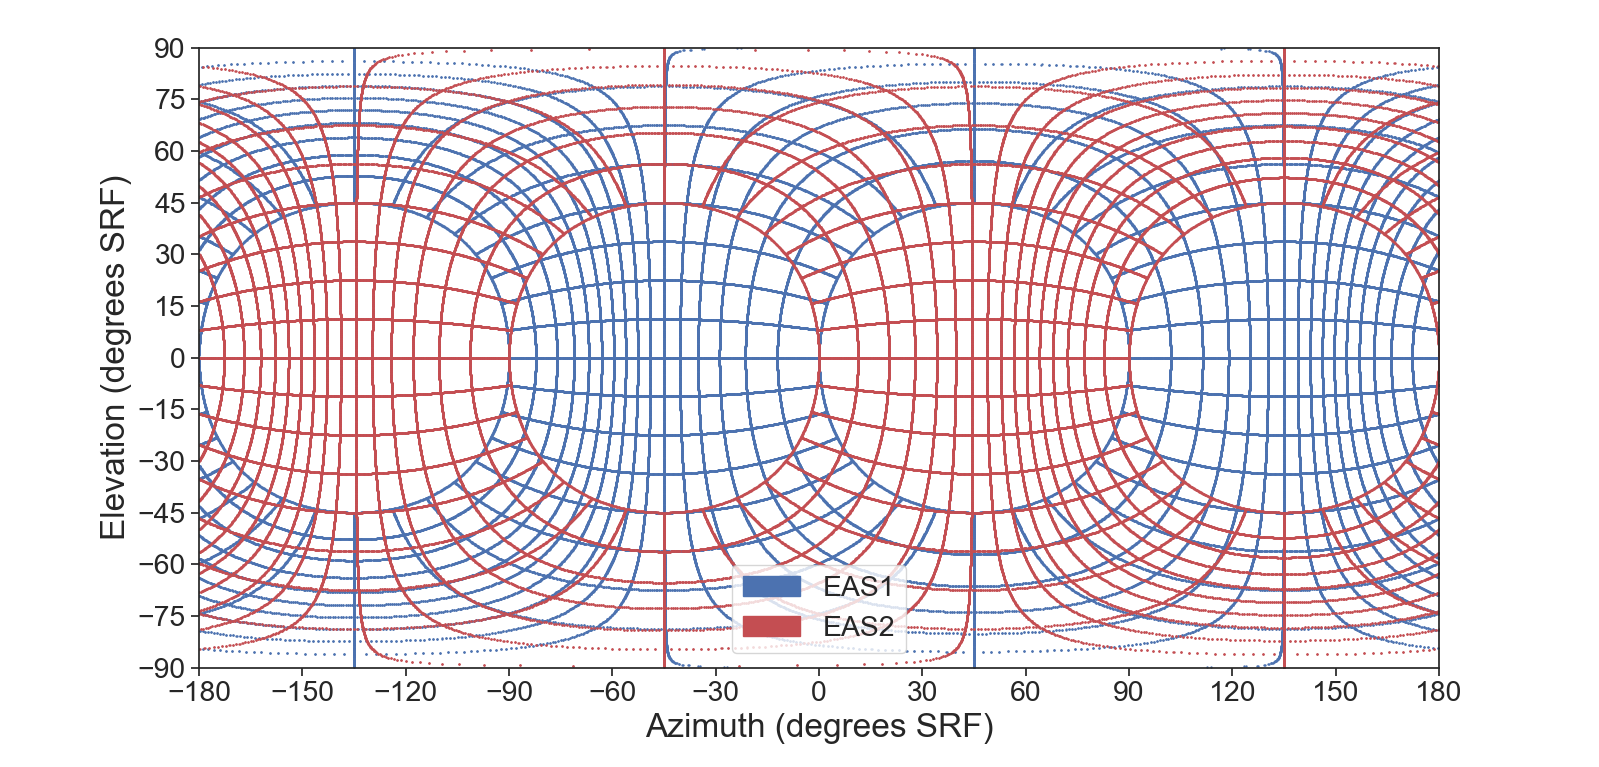
\includegraphics[width=1.2\linewidth]{figures/all bins.png}
    \caption{A plot  of EAS1 (blue) and EAS2 (red) elevation and azimuth bins projected onto the sky in spherical spacecraft reference frame (SRF) coordinates. Note that \q{elevation} and \q{azimuth} as labelled in the axes refer to the coordinates in SRF; \textit{not} the elevation/azimuth in the sensor head frames (e.g. Figure \ref{fig: EAS schematic}). Note also that between EAS1 and EAS2, it is possible to cover the entire sky with some overlap.}
    \caption*{Image Source: Author's own work}
    \label{fig: all bins}
\end{figure}

\begin{figure}[h!]
    \centering
    \centerfloat
    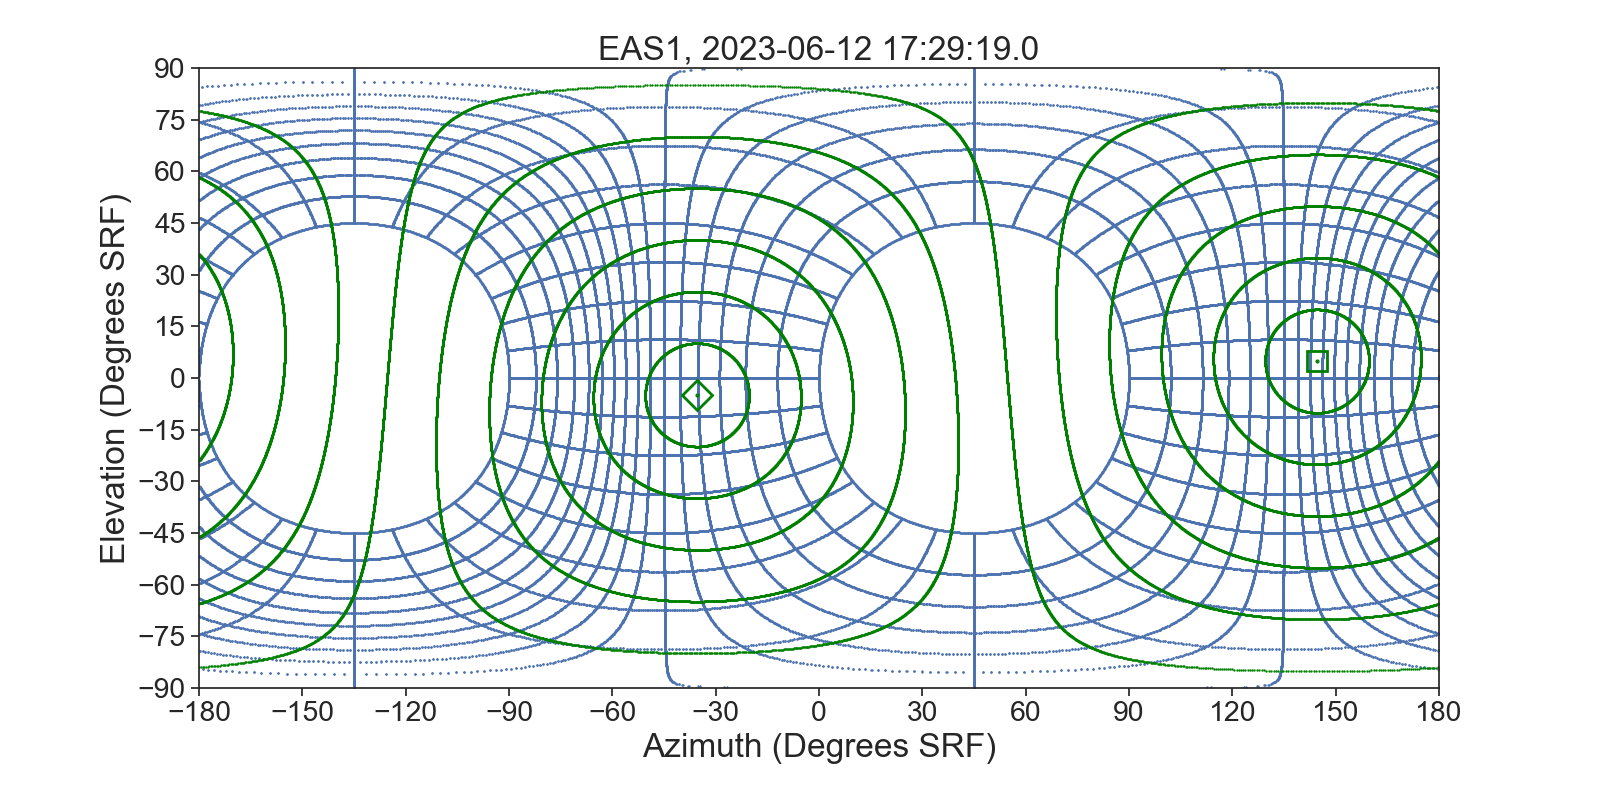
\includegraphics[width=1.2\linewidth]{figures/fullcontours_justeas_noselection.png}
    \caption{Another plot of projected EAS1 elevation and azimuth bins in SRF overlaid with a magnetic field vector from MAG. The point parallel to the vector is indicated by the green diamond, and the point anti-parallel to the vector is indicated by the green square. The green contours represent pitch angles in 15\degree increments from 15\degree to 165\degree. MAG vector data are taken from the Solar Orbiter Archive, from a period of data collection on 12th June 2023. }
    \caption*{Image Source: Author's own work}
    \label{fig: normal - full contours}
\end{figure}


\newpage
\subsection{EAS Burst Mode} \label{EAS Burst Mode}

EAS Burst Mode data are typically collected over periods of \(\sim5-15\)minutes, once per day. Compared to Normal Mode at full cadence, full Burst Mode PADs can be acquired after sampling only 2 of the 16 elevation bins in the sky, resulting in a theoretical \(8\times\) improvement in sample cadence (8Hz at \(\sim0.125\)s/sample). Compared to other typical Normal Mode cadences of 4s/sample, 10s/sample, or 100s/sample, the improvement can be as good as \(32\times\), \(80\times\), or \(800\times\) respectively. The Burst Mode PAD pipeline can be summarised as follows\cite{owen2021}:

\begin{enumerate}
    \item Acquire a MAG vector at 8Hz,
    \item Transmit the MAG vector directly to EAS via the onboard \q{S20} data link,
    \item Select the EAS head that has the MAG vector closest to the center of its FOV,
    \item For that head, select the \textbf{2} elevation bins that contain the parallel and antiparallel MAG vector in their respective FOVs,
    \item Acquire a partial-sky VDF with 64 energy bins \(\times\) 2 selected elevation bins \(\times\) 32 azimuth bins at 8Hz,
    \item Downlink EAS VDF to ground,
    \item Re-bin EAS VDF on ground, yielding a full PAD.
\end{enumerate}

\begin{figure}
    \centering
    \centerfloat
    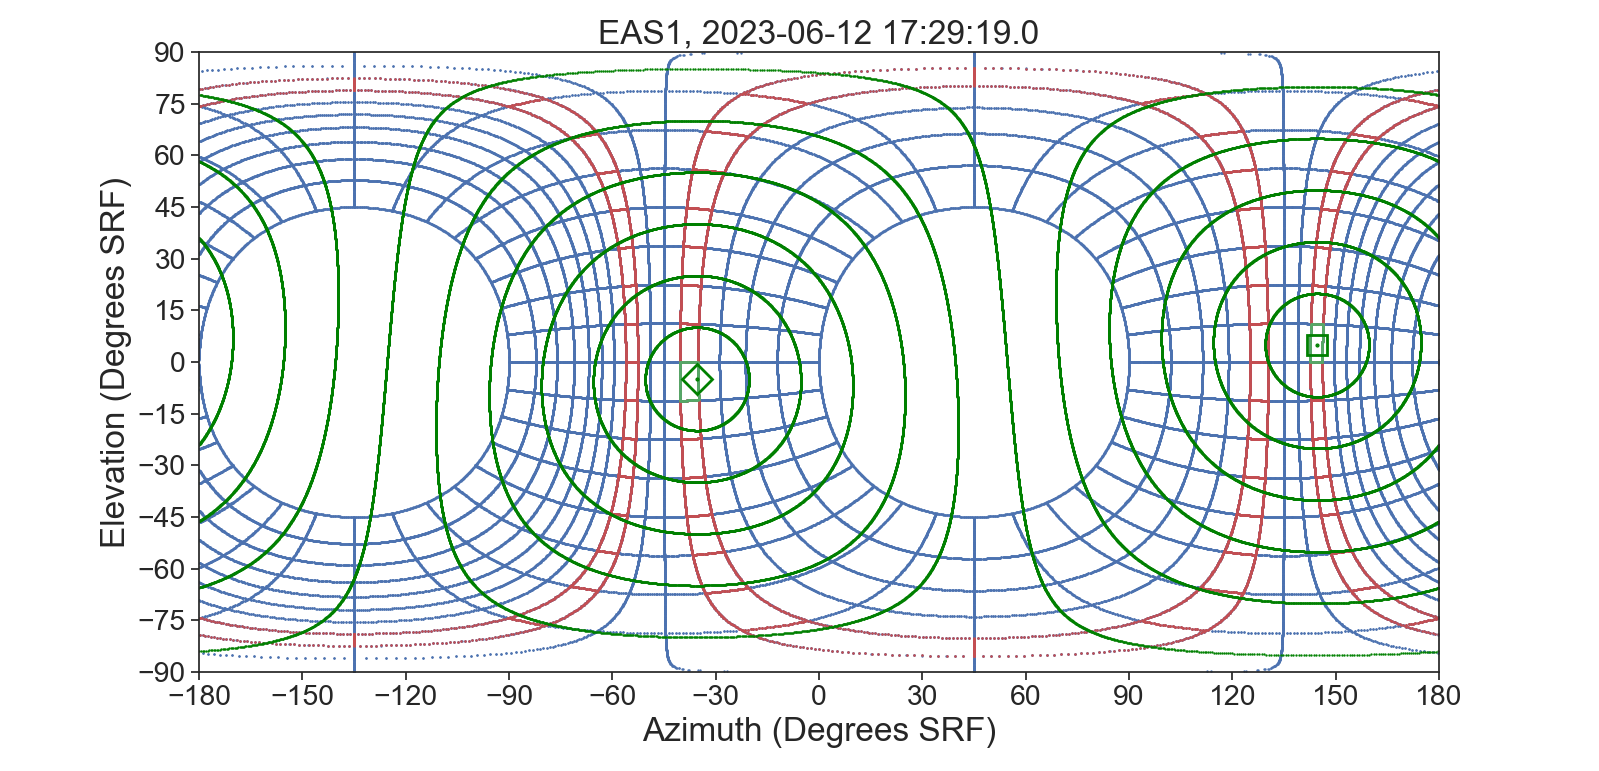
\includegraphics[width=1.2\linewidth]{figures/fullcontours_justeas_yesselection.png}
    \caption{A similar plot to Figure \ref{fig: normal - full contours}. Additionally, the bands of EAS1 elevation bins containing the parallel and antiparallel magnetic field vectors are highlighted in red, and the elevation and azimuth pixels containing the same vectors are highlighted in green. MAG vector data are taken from the Solar Orbiter Archive, from a period of data collection on 12th June 2023. }
    \caption*{Image Source: Author's own work}
    \label{fig: normal - full contours + selection}
\end{figure}

For a more detailed description, consider Figure \ref{fig: normal - full contours + selection}. This figure shows the same bins, vectors, and pitch angle contours as Figure \ref{fig: normal - full contours}, but the bands of elevation bins containing the parallel and antiparallel magnetic field vectors are highlighted in red, and the pixels containing the parallel and antiparallel magnetic field vectors are highlighted in green. Note that each elevation band is separated into azimuthal bins. Within the elevation band containing the parallel vector, as angular distance increases from the azimuthal bin/pixel containing the vector, successive azimuthal bins are crossed by higher and higher pitch angles, culminating in an angle \(\alpha\geq90\degree\). Conversely, as angular distance increases from the azimuthal bin containing the antiparallel magnetic field vector, successive azimuthal bins are crossed by lower and lower pitch angles, culminating in an angle \(\alpha\leq90\degree\). For the sensor head containing the magnetic field vector in its FOV, the geometry of the sensor heads guarantees that this is always true\cite{owen2021}; the two opposite sides of a hypothetical elevation bin at 0\degree\ elevation would reach a maximum of \(\sim180\degree\) apart, and the opposite sides of an elevation bin at \(\pm45\degree\) would reach a minimum of \(\sim90\degree\) apart. Therefore, by \q{steering} EAS to sample each azimuthal bin across only the two highlighted elevation bands, it is possible to sample electrons with a full range of 0\degree-180\degree\ pitch angles. With the assumption of gyrotropy, this represents a full PAD (e.g. Figure \ref{fig: PAD example}). Since the 32 azimuth bins at each elevation are sampled simultaneously, this costs no additional time, resulting in an eight-fold sample time reduction.
\\

To sample only the elevation bins containing the parallel and antiparallel magnetic field vector, EAS must first be told the orientation of the magnetic field. On Solar Orbiter, this is communicated via the \q{S20 inter-instrument communications link} which is transmitted by the MAG Instrument Control Unit (MAG-ICU) and received by the SWA-DPU\cite{owen2021}\cite{owen2020}\cite{horbury2020}. Once received, SWA-DPU must select the EAS head that has the magnetic field closest to the center of its FOV, which is equivalent to finding the smallest angle between the vector and the sensor head aperture center-plane\cite{owen2021}.
\\

While Burst Mode boasts far-superior time resolution, it is also vulnerable to errors that Normal Mode avoids. By virtue of the fact that Burst Mode uses MAG data transmitted directly over the S20 data link, it therefore also does not benefit from post-processing of MAG data on the ground. Errors that may result in a discrepancy between the vectors used to \q{steer} EAS and the \q{more-correct} ground vectors include: 
\begin{itemize}
    \item Un-calibrated offset drift in MAG measurement axes, which may be more significant during the period leading up to a routine calibration update\cite{owen2021}\cite{horbury2020}.
    \item Data latency in the S20 inter-instrument link itself, which may be inherent and/or exaggerated  by periods of heavy data traffic\cite{owen2021}.
\end{itemize}

When errors like these cause EAS to select incorrect elevation and azimuth bins in Burst Mode, this can lead to missing and mislabelled PAD data. The next chapter describes the methods applied to analyse the impact of these and other errors on Burst Mode PAD accuracy and completeness, and to encapsulate some of that impact in the form of a \q{completeness score}.

